\documentclass[10pt, a4paper]{article}
\usepackage[T1]{fontenc}
\usepackage[utf8x]{inputenc}
\usepackage{ifpdf}
\usepackage{graphicx}
\usepackage{array}
\usepackage{multirow}


\usepackage{listings}	% For program listings.
\usepackage{color}
\definecolor{dkgreen}{rgb}{0,0.6,0}
\definecolor{gray}{rgb}{0.5,0.5,0.5}
\definecolor{mauve}{rgb}{0.58,0,0.82}
\lstset {
	language=Matlab,			  		% The language of the code.
	basicstyle=\footnotesize,			% The size of the fonts that are used for the code.
	numbers=left,						% Where to put the line-numbers.
	numberstyle=\tiny\color{gray},		% The style that is used for the line-numbers.
	stepnumber=1,						% The step between two line-numbers. If it's 1, each line will be numbered.
	numbersep=5pt,						% How far the line-numbers are from the code.
	backgroundcolor=\color{white},		% Choose the background color. You must add \usepackage{color}.
	showspaces=false,					% Show spaces adding particular underscores.
	showstringspaces=false,				% Underline spaces within strings.
	showtabs=false,						% Show tabs within strings adding particular underscores.
	frame=single,						% Adds a frame around the code.
	rulecolor=\color{black},			% If not set, the frame-color may be changed on line-breaks within not-black text (e.g. commens (green here)).
	tabsize=2,							% Sets default tabsize to 2 spaces.
	captionpos=t,						% Sets the caption-position to bottom.
	breaklines=true,					% Sets automatic line breaking.
	breakatwhitespace=false,			% Sets if automatic breaks should only happen at whitespace.
	title=\lstname,						% Show the filename of files included with \lstinputlisting;  also try caption instead of title.
	keywordstyle=\color{blue},			% Keyword style.
	commentstyle=\color{dkgreen},		% Comment style.
	stringstyle=\color{mauve},		  	% String literal style.
	escapeinside={\%*}{*)},			  	% If you want to add a comment within your code.
	morekeywords={*,...}			  	% If you want to add more keywords to the set.
}

\newcommand{\matlab}{\small{\emph{MATLAB\textsuperscript{\textregistered}}}}

\title{Numerical Analysis for Computer Scientists\\ FMN011, Lund University 2012\\ Project \#2\\ Finding the line strength of stars for an astronomer}
\date{}
\author{Erik Westrup, \texttt{<ada09ewe@student.lu.se>}}

\begin{document}
\begin{titlepage}
\maketitle

\thispagestyle{empty}
\end{titlepage}
\setcounter{page}{2}

\section{Introduction and Problem Background}
This project is about solving real-world problems with their accompanied complexities and ambiguities. The best method must be determined and its limitations and possible errors must be known. In this project intensity of light from stars will be studied. Stars produces a continuous curve of light over a range of frequencies called the \emph{spectrum} for that star. It can be measured in \emph{relative intensity} ($\frac{\mathrm{W}}{\mathrm{m}^2\times\mathrm{Hz}}$) as a function of the frequency (Hz) which is defined as the spectrum. What is interesting is that the surrounding gases of a star will either absorb (cold gas) or emit (warm) light which is visible at discrete fixed frequencies in the spectrum as \emph{spectral lines}. By identifying these spectral lines the components of the star can be found  because each chemical composition have a unique fingerprint of discrete frequencies \cite{astronotes1} \cite{astronotes2}. % TODO is Hz in the numerator or denominator?

In this project a measured continuous spectrum for a star is given which contains six spectral lines evenly divided in absorption lines and emissions lines. The task for this project is to find the total intensity for each of these spectral lines called the \emph{line strength} measured in $\frac{\mathrm{M}}{\mathrm{m}^2}$ \cite{linestrength}. This is achieved by finding the area under the curve at the peak-frequencies i.e. integrating the relative intensity over these frequencies. % TODO why do you want the area?

The given data is a file with $4000$ measurements of \emph{Specific Intensity} in $\frac{\mathrm{W}}{\mathrm{m}^2\times \mathrm{Hz}}$ at frequencies in the range $[3.50\times10^{14}, 4.29\times10^{14}]$.

\section{Numerical Considerations}

\section{Results \& Analysis}
The first thing to do is, as always, to get an understanding of what are the given. Since studying the raw data is hard a graphical plot over the curve is desired to grasp the main characteristics of what we have. The relative intensity spectrum can be seen in figure \ref{fig+rellspec} and the spectrum itself in figure \ref{fig+spec}. In these two plots the six spectral lines are clearly visible. Just for the interest the intensities are also show as a function of the wave lengths in figure \ref{fig+specwave} using the \matlab{} function \emph{spectrumLabel}\cite{spectrumLabel}.


\begin{figure}[hbt]
\begin{center}
\ifpdf
	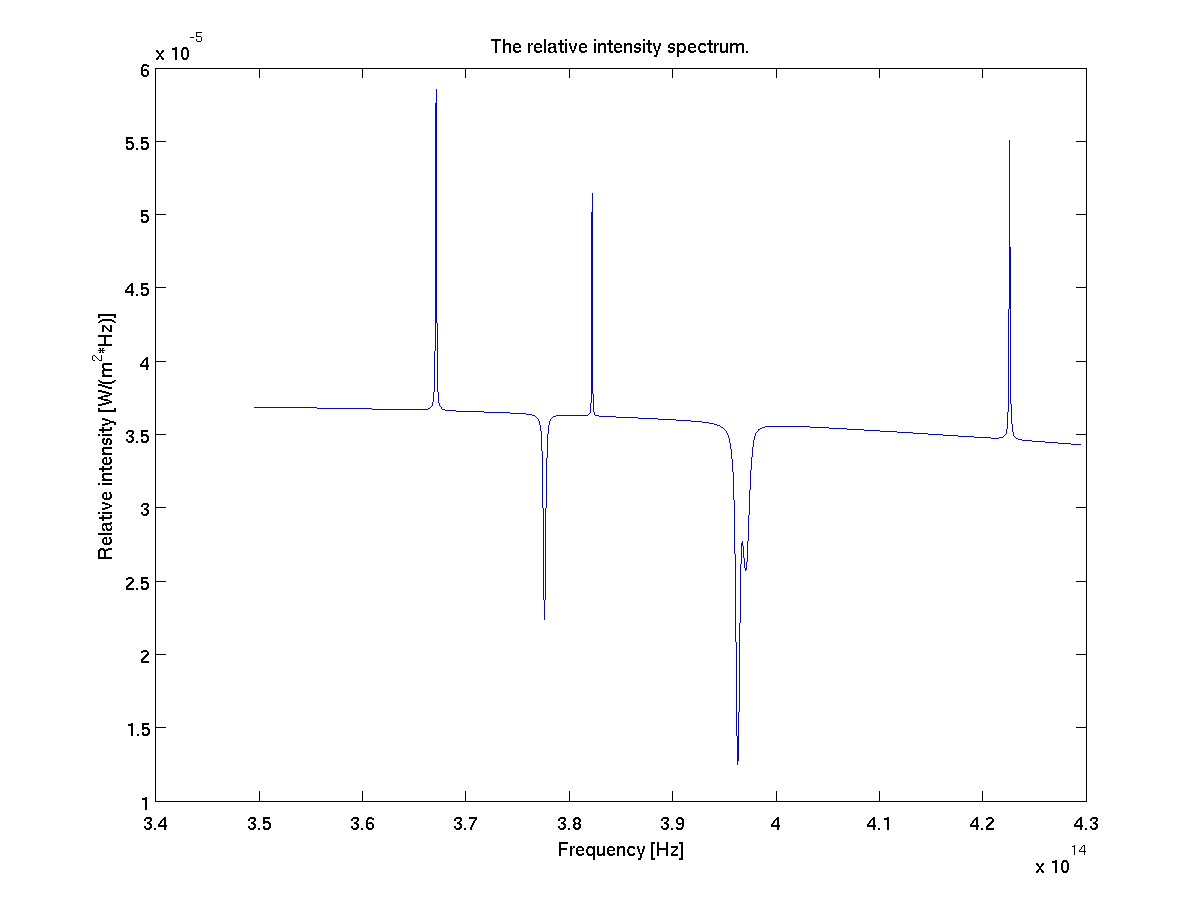
\includegraphics[width=\linewidth]{../img/spectrum_relative.png}
\else
	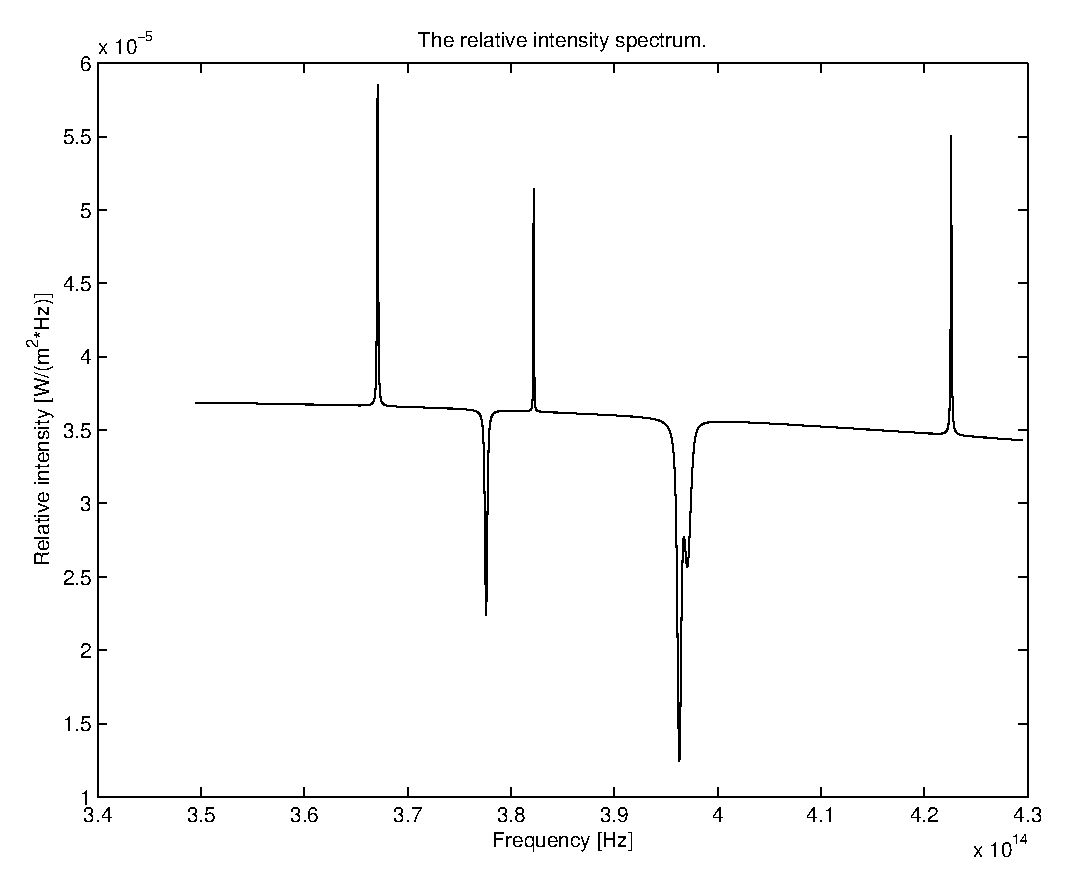
\includegraphics[width=\linewidth]{../img/spectrum_relative.eps}
\fi
\end{center}
\caption{}
\label{fig+rellspec}
\end{figure}

\begin{figure}[hbt]
\begin{center}
\ifpdf
	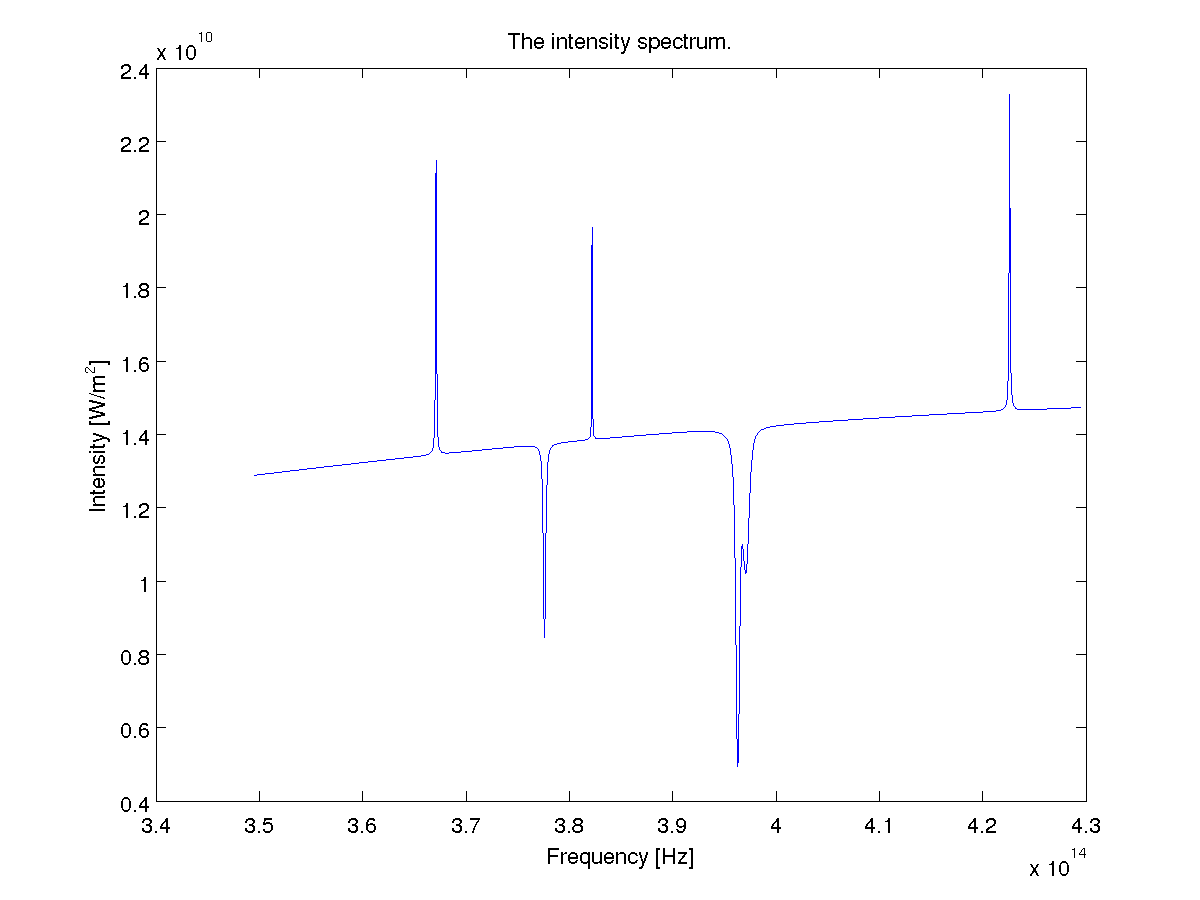
\includegraphics[width=\linewidth]{../img/spectrum.png}
\else
	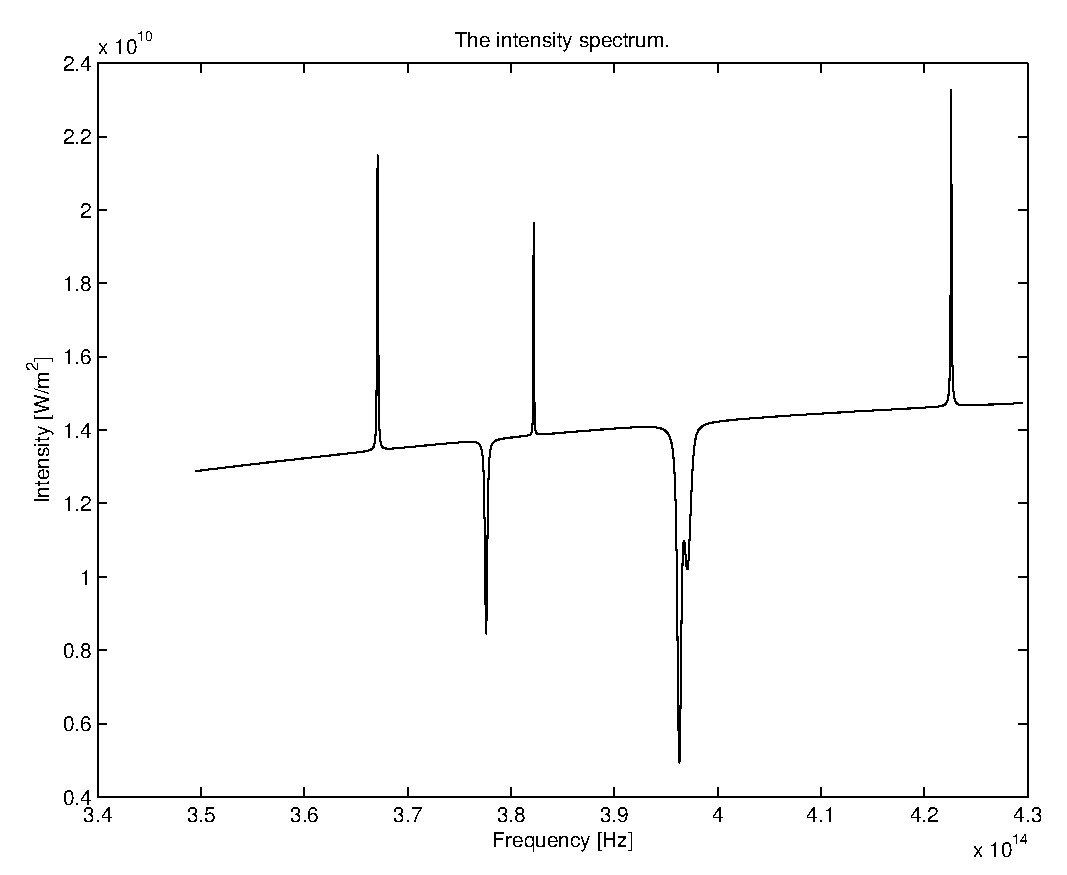
\includegraphics[width=\linewidth]{../img/spectrum.eps}
\fi
\end{center}
\caption{}
\label{fig+spec}
\end{figure}

\begin{figure}[hbt]
\begin{center}
\ifpdf
	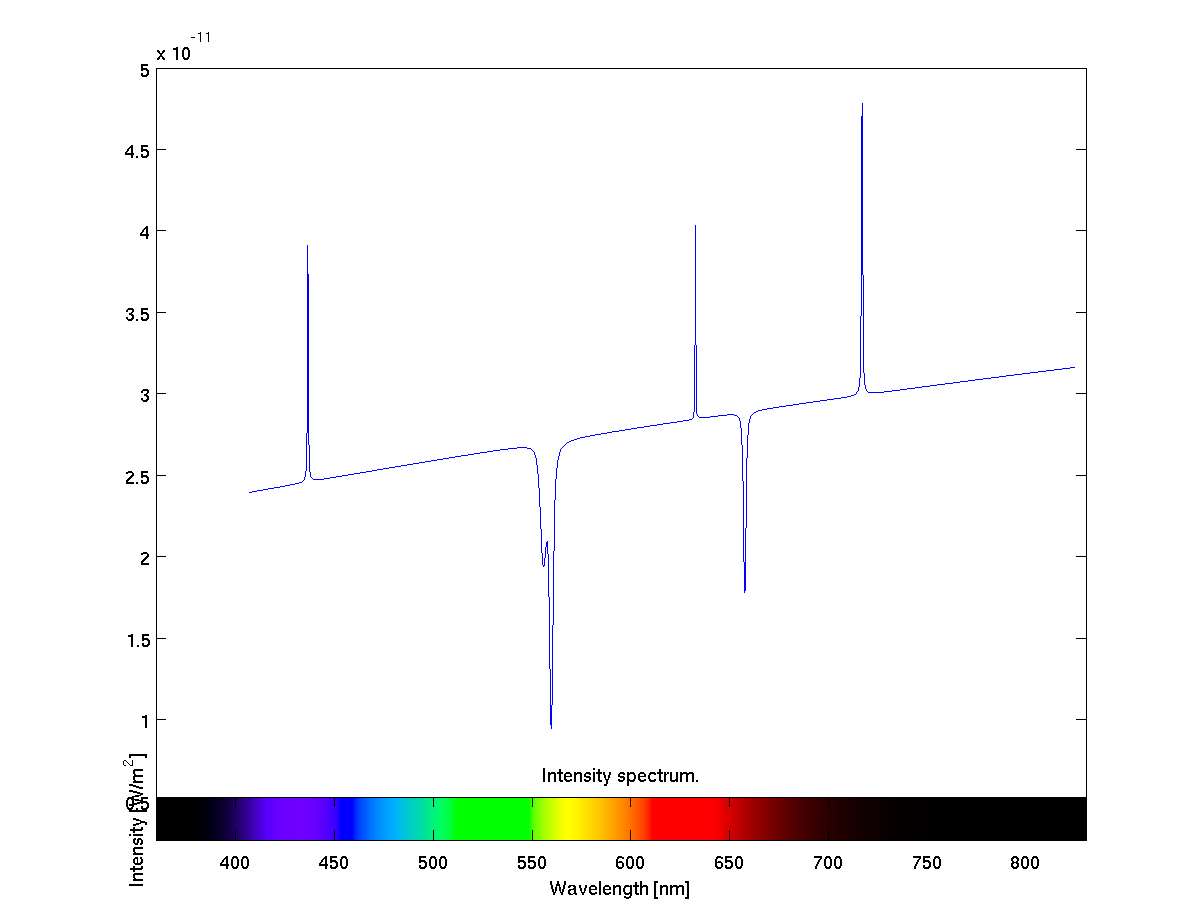
\includegraphics[width=\linewidth]{../img/spectrum_wave.png}
\else
	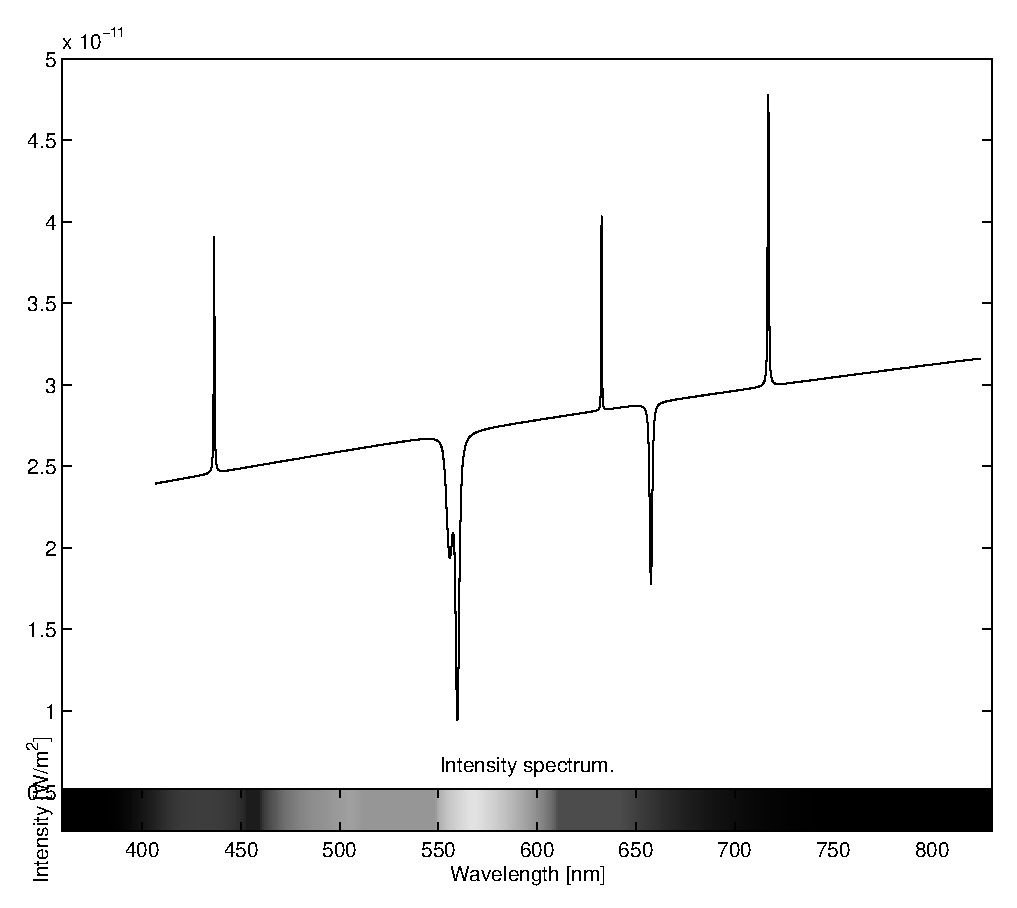
\includegraphics[width=\linewidth]{../img/spectrum_wave.eps}
\fi
\end{center}
\caption{}
\label{fig+specwave}
\end{figure}
\clearpage



\section{Lessons Learned}
From this project several theoretical understandings are gained.
\begin{itemize}
	\item \ldots
\end{itemize}

\begin{itemize}
	\item \ldots
\end{itemize}


\section{Acknowledgments}

I worked tightly with Oscar Olsson, Tommy Ivarsson and Jonas Klauber.

\bibliography{references}{}
\bibliographystyle{ieeetr}

\newpage
\section*{Appendix}
\appendix
\section{Program listings} \label{appendix+programs}
Here the \matlab{} functions and scripts used to achieve the results above are listed.

\subsection{Scripts}
The following scrips are the drivers for producing the results found in this report.

\lstinputlisting{src/pr2.m}

\subsection{Functions}
The following functions implements the algorithms and the rest serves as helper functions to these algorithms and the scripts. To distinguish these from other \matlab{}-functions in the global namespace these reside in a own package called \emph{pr2}.

%\lstinputlisting{src/+pr1/init_task.m}

\end{document}
